
\subsection{Architettura logica}
\label{sec:logical-arch}
Come già anticipato in Sezione~\ref{sec:func-req},
il sistema dovrà gestire due tipologie di informazioni.\\

La descrizione del grafo principale e le caratteristiche scelte
in fase di configurazione simulano la collocazione dei robot in
un ambiente fisico reale che si mantiene costante: dovranno dunque
essere accessibili dall'intero sistema in qualunque momento,
ma non potranno essere utilizzate
nella loro totalità
per risolvere la ricerca della query.
Avremo un modulo `\textbf{\emph{DSDataFacade}}' che conterrà:
\begin{itemize}
\item \emph{mainGraph}: il grafo caricato dall'utente rappresentante
  l'ambiente totale;
\item \emph{numRobot}: il numero di robot collocati nella mappa;
\item \emph{occupied}: l'elenco dei nodi in cui i robot sono posizionati.
\end{itemize}
I primi due campi della `\emph{DSDataFacade}' sono costanti e vengono
istanziati in fase di inizializzazione: in questa fase si provvede anche
a inizializzare in modo random il vettore `\emph{occupied}'. Quest'ultimo
potrà essere modificato durante l'esecuzione del sistema in seguito allo
spostamento dei robot.
Solo il modulo di visualizzazione potrà accedere alla `\emph{DSDataFacade}'
richiedendo la posizione dei robot, permettendo di monitorare
il loro movimento: non è infatti ammesso ai singoli robot di conoscere
la posizione degli altri né il loro numero complessivo per risolvere
il problema.\\

Gli altri moduli del sistema sono volti a implementare i
ruoli coinvolti in un'implementazione fisica reale.
Utilizzando la terminologia di \emph{Akka}, questi costituiscono
\emph{attori}, ovvero astrazioni con comportamento fortemente coeso
che implementano determinate funzionalità innescate dallo scambio di
messaggi. Gli attori si possono trovare su diversi \emph{Actor Systems},
che rappresentano nodi distinti della rete.

Ogni \textbf{robot} è un Actor System su cui sono in esecuzione più attori:
\begin{itemize}
\item `\emph{DSRobot}': è l'attore principale; viene costruito specificando
  il nodo in cui è stato posizionato in fase di inizializzazione.
  Accede alla `\emph{DSDataFacade}' per caricare in memoria la vista
  `\emph{myView}' a partire da `\emph{myNode}'
  del grafo principale, simulando in questo modo l'effettiva
  acquisizione di conoscenza tramite sensori dell'ambiente.

  Quando una query viene sottoposta al sistema, `\emph{DSRobot}' riceve
  un messaggio che impone di creare un attore figlio
  `\emph{DSQueryChecker}'.
  La definizione di un'adeguata gerarchia tra attori si rivela fondamentale
  per poter gestire i fallimenti: infatti il processo padre sarà
  responsabile dei figli.
\item `\emph{DSQueryChecker}': sono gli attori figli costruiti in un
  robot. Il loro comportamento è estremamente specializzato alla
  verifica e alla gestione di una determinata query. Sono presenti in numero pari
  al numero delle query in circolazione in quel momento e vengono
  distrutti dal processo padre appena la query che gestisono ha raggiunto
  un risultato.
\end{itemize}

Ogni \textbf{client} che si interfaccia al sistema costituisce un nuovo Actor System.
In esso c'è un solo attore `\emph{DSClusterInterfaceActor}':
esso deve essere il punto di accesso al cluster per l'utente.\\
In relazione al cluster deve mandare la query che l'utente
sottopone e ottenere da questo il risultato della computazione;
deve essere informato anche degli eventuali fallimenti
riscontrati tra i robot per poter ripresentare la query.\\
Per gestire l'interfaccia con l'utente potrà accedere alle informazioni
presenti in ogni host, contenute nel modulo `\emph{DSCluster}'.
Tale modulo è condiviso con il modulo di visualizzazione grafica
`\emph{DSView}' che si occupa di settare i dati e i comandi dell'utente.
In particolare verrà memorizzato in `\emph{DSCluster}' l'elenco delle
query sottoposte da quel particolare client con i relativi
risultati.

Si noti che tali Actor System non conoscono la posizione degli altri,
dunque non sarà possibile mandare messaggi one-to-one,
ma si dovrà sempre passare per meccanismi di comunicazione che svincolano
dalla necessità di conoscere la località dei destinatari.

\subsection{Protocollo e algoritmo}
\label{sec:protocols}

Le comunicazioni tra le varie componenti del sistema sfruttano
principalmente il meccanismo di
\emph{Distribuited Publish Subscribe in Cluster} offerto da Akka.
Esso consente di comunicare con un insieme di attori che si
dichiarano interessati a un determinato topic senza che il mittente
conosca gli \emph{ActorRef} dei destinatari. Per questi motivi
risulta una funzionalità particolarmente adatta al sistema in questione
perché garantisce una massima location transparency tra i diversi
Actor System.
Gli attori membri di un cluster possono iscriversi a un \emph{path}
oppure a un \emph{subject}; l'invio di un messaggio tramite il
\emph{DistribuitedPubSubMediator} di Akka può essere eseguito in
modalità: a) \emph{SendToAll} / \emph{Publish}, il messaggio viene
ricevuto da tutti gli attori iscritti, eventualmente settando il
parametro \emph{allButSelf} che esclude il mittente;
b) \emph{Send}, il messaggio viene ricevuto da un solo attore
iscritto al cluster, eventualmente specificando la preferenza
\emph{location affinity}.

\subsubsection*{Inizializzazione del sistema:}
In Figura~\ref{fig:UML-classes} mostriamo le relazioni di
dipendenza tra le componenti descritte nella precedente sezione.
\emph{DSCluster} contiene un vettore indicante gli host
permettendo alla \emph{DSView} (che possiede) di simulare
la connessione di nuovi client.
Il modulo di visualizzazione invoca i suoi metodi per innescare
una nuova query o impostare i parametri del sistema.
Durante la fase di inizializzazione,
il metodo \texttt{actorSystemInitialization()} crea gli Actor
System per i robot
%~\footnote{
%  Poiché la simulazione lavora in locale, i vari Actor System sono
%  distinti in quanto in ascolto ognuno su porte diverse.}
un numero pari a quello definito dall'utente,
e crea in essi l'attore principale \emph{DSRobot}. Viene inoltre
creato l'Actor System e il relativo \emph{DSClusterInterfaceActor}
per il primo host connesso.

Gli attori \emph{DSRobot} si iscrivono al cluster in ascolto su un
path dedicato alle comunicazioni all'intero insieme di robot;
mentre i \emph{DSClusterInterfaceActor} si iscrivono a un topic
specifico per le comunicazioni verso il corrispondente host.

\subsubsection*{Sottomettere una nuova query:}
L'algoritmo viene innescato quando l'utente sottopone una query $\cQ$
al sistema, caricandola in un qualunque momento
dopo la sua configurazione. La \emph{DSView} invoca allora
il metodo \texttt{startNewComputation()} del \emph{DSCluster}:
in questo si provvede a versionare la query,
ottendo un identificativo univoco.
Viene dunque madato un messaggio
\texttt{DSStartQueryCheck} sul path su cui è in ascolto
il \emph{DSClusterInterface} relativo all'host che ha sottoposto
la query: il messaggio contiene la versione serializzata
della query con l'identificativo calcolato.
Come mostrato in Figura~\ref{fig:UML-messages},
quando riceve questo messaggio il \emph{DSClusterInterfaceActor},
manda in SendAll all'intero cluster di robot un messaggio
\texttt{DSCreateQueryCheckers} contenente il solo identificativo della
query: in un \emph{DSRobot} la routine associata alla ricezione
di questo messaggio crea un attore figlio \emph{DSQueryChecker}.

I vari \emph{DSQueryChecker} ricavano dal padre la vista
conosciuta del grafo $\cV$ e il nodo sul quale sono posizionati;
sono inizializzati in ascolto sul path definito dall'identificativo
della query: in questo modo sarà possibile gestire
distintamente le comunicazioni relative alle diverse versioni delle
query sottoposte senza rischio di interferenza.

\`E il \emph{DSClusterInterface} a mandare in Send per primo
il messaggio \texttt{TryNewQuery} sul path dei \emph{DSQueryChecker}.
La query viene così ricevuta da un attore alla volta: esso provvede
a confrontare la query con la propria conoscenza parziale del grafo.
Questa computazione corrisponde al cuore dell'algoritmo del
subgraph isomorphism problem e verrà analizzato in dettaglio
successivamente.
Se rimangono degli elementi da verificare, l'attore manda allora
un nuovo messaggio \texttt{TryNewQuery} contenente la query ridotta
al path, dopo essersi disinscritto da esso.

Quando il query checker di ogni robot ha visualizzato e partecipato
alla verifica della query, ovvero quando non c'è più alcun destinatario
iscritto al path, ma la query non è stata ancora interamente verificata,
lo stato uscente è \texttt{DONTKNOW}.
In caso invece si riesca a raggiungere il risultato di \texttt{MATCH}
o \texttt{FAIL}, la computazione viene interrotta prima di passare
per ogni robot. Il termine della computazione comprende l'invio
in SendAll ai robot un messaggio \texttt{DSEndQuery} e al cluster
un messaggio \texttt{DSMissionAccomplished}:
il risultato può essere così trasmesso all'utente e i \emph{DSRobot}
provvedono a terminare i processi figli relativi alla query terminata.

Quando al \emph{DSCluster} giunge il risultato della query,
questo provvede a comunicarlo all'utente tramite il modulo di
visualizzazione. Viene mantenuto in memoria l'elenco delle
query sottoposte fino a quel momento che l'utente può visualizzare
in elenco: nel caso il risultato sia \texttt{DONTKNOW}, affiancata
alla query e al suo identificativo, si mantiene anche la sua versione
(ridotta) che ancora manca da verificare. In questo modo
l'utente può ritentare di verificare la query solo nelle parti
ancora da controllare.

In qualunque momento l'utente può far muovere i robot cercando di
aumentare la somma della conoscenze parziali del grafo: questo
avviene inviando tramite il \emph{DSClusterInterfaceActor} un
messaggio \texttt{DSMove} sul path dei robot.
Ognuno di questi allora sceglie un nodo adiacente
a quello in cui è attualmente posizionato e carica in memoria
una nuova vista spostandosi in esso.
Questo richiede necessariamente un accesso al `\emph{mainGraph}' della
\emph{DSDataFacade} che simula l'effettiva acquisizione di
nuova conoscenza: durante questa fase, per simulare il limite di
memorizzazione dei robot, vengono rimossi da `\emph{myView}'
i nodi conosciuti due passi indietro.
La scelta del nodo su cui spostarsi è random, in quanto il robot
non ha modo di scegliere il nodo più informativo non conoscendo
il grafo né tutte le query che sono in fase di verifica:
tra la scelta degli adiacenti però viene escluso il nodo su cui
si trovava al passo precedente, memorizzato come
`\emph{lastStep}', per evitare quantomeno che ritorni sui suoi passi.

\subsubsection*{Gestione dei fallimenti dei \emph{DSQueryChecker}:}
Come mostrato in Figura~\ref{fig:UML-messages},
per proteggersi da fallimenti, ulteriori messaggi possono essere
inviati: poiché solo un query checker alla volta possiede la query
più aggiornata, se questo fallisse mentre la sta verificando,
non ci sarebbe modo di recuperarla.
All'inizio e alla fine del lavoro critico invia rispettivamente i
messaggi \texttt{DSStartCriticalWork} e \texttt{DSEndCriticalWork}
al processo padre: questo potrà mantenere i riferimenti dei
figli conoscendo il loro stato di esecuzione:\begin{itemize}
\item waiting : è iscritto al cluster ma non ha ancora ricevuto la query;
\item critical : sta verificando la query;
\item done : ha già contribuito con le sue informazioni alla verifica
  della query e si è disinscritto.
\end{itemize}
Se un \emph{DSQueryChecker} termina, grazie al sistema gerarchico
formatosi, il padre viene informato e può controllare in quale fase del
lavoro si trovava l'attore.

Se questo era in `waiting' allora si occupa
di ricrearlo semplicemente così che si possa iscrivere al path ed
attendere il suo turno.

Se l'attore era invece in fase critica, la query è stata persa durante
la verifica: occorre dunque farla ricominciare inviando un messaggio
\texttt{DSRetryQuery} al cluster che ha fatto richiesta.
Grazie al sistema di versionamento e al fatto di utilizzare tale
identificativo come percorso su cui collocare i \emph{DSQueryChecker},
il robot può recuperare dal nome del percorso su cui è morto il figlio
il nome della query e l'host a cui richiederla.
Viene inoltre inviato un messaggio \emph{DSEndQuery} ai robot
per terminare anche gli altri query checker che altrimenti rimarrebbero
sospesi.

Infine, se l'attore termina dopo aver già contribuito alla verifica
della query, allora non è necessario riavviarlo.

In tutti i casi, l'utente non viene informato di questo tipo di
fallimenti in quanto il sistema riesce autonomamente a gestirli
facendo ripartire la ricerca dall'ultimo risultato ottenuto.

\subsubsection*{Gestione dei fallimenti dei \emph{DSRobot}:}
Questo tipo di fallimenti risulta particolarmente critico per
l'esecuzione dell'algoritmo, inoltre è ragionevole pensare che
l'utente voglia essere informato della morte di un robot.
Per simulare l'immediata sostituzione del robot nel cluster,
possiamo lasciare che sia la strategia di fault tollerance di default
di Akka a reinizializzarlo: specificando il metodo \texttt{postRestart}
si può inviare il messaggio \texttt{DSRobotFailureOccurred}
in \emph{Publish} al topic a cui tutti i
\emph{DSClusterInterfaceActor} sono iscritti: in questo modo tutti gli
host saranno informati che un robot è morto ed è stato sostituito.
Viene inoltre inviato lo stesso messaggio a tutti i
robot per terminare effettivamente tutte le computazioni attive
in quel momento.

%%%%%%%%%%%%%%%%%%%%%%%
\begin{figure}[ht!]
\centering
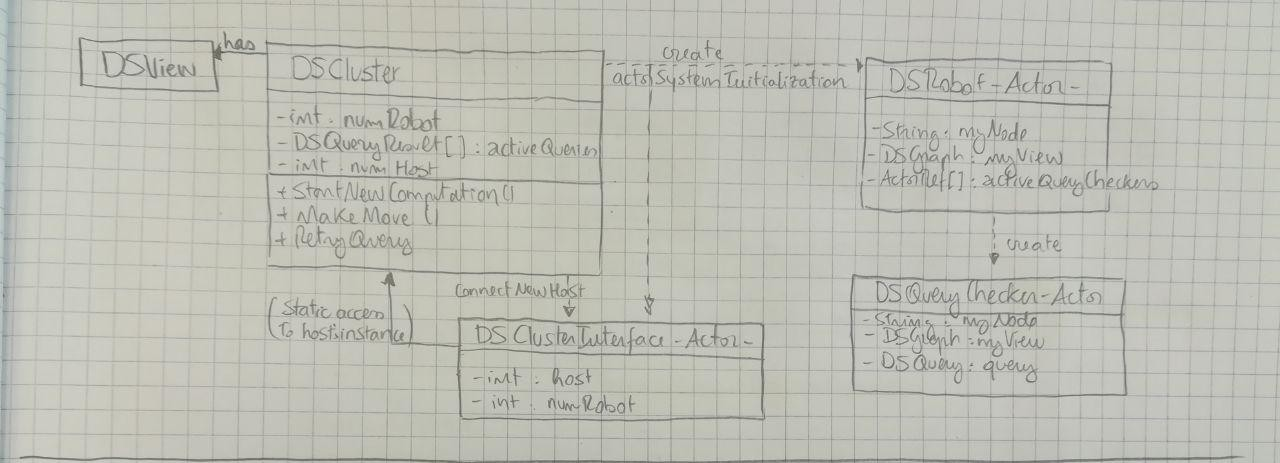
\includegraphics[width=\textwidth]{UML-classes.jpg}
\caption{\label{fig:UML-classes}
\coanote{FIXME: add the UML from photo...}
}
\end{figure}
%%%%%%
\begin{figure}[ht!]
\centering
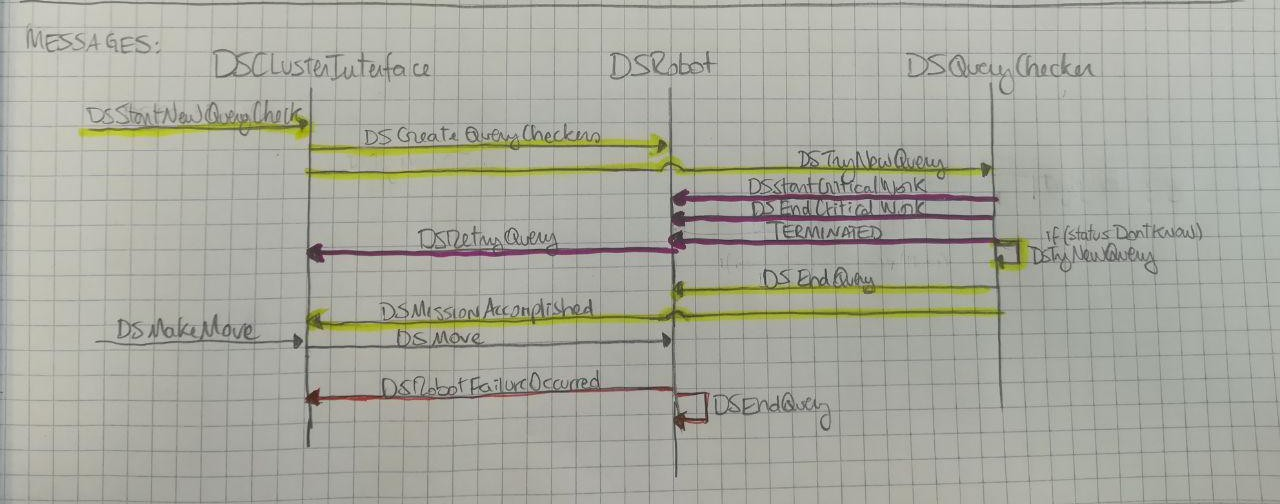
\includegraphics[width=\textwidth]{UML-messages.jpg}
\caption{\label{fig:UML-messages}
  \coanote{FIXME: add the UML from photo...
    cassu! c'è un errore: l'arco di messaggi tra DSRobot e DSRobot rosso
  è DSRobotFailureOccurred, e *non* DSEndQuery.}
}
\end{figure}

%%%%%%%%%%%%%%%%%%%%%%
\[
\adj{v}{\cG} = \bigl\{\, v' \bigm| (v, v') \in E,
\ \cG = (\Vset, E) \,\bigr\}.
\]
%%%%%%%%%
\begin{algorithm}
  \caption{Verifica e riduzione di una query: dati in input
    un grafo $\cV$ rappresentante la conoscenza parziale del grafo,
    il nodo $v$ nel quale si è posizionati e
    una query $\cQ$, restituisce \texttt{MATCH} / \texttt{FAIL}
    / \texttt{DONTKNOW} come definito in Sezione~\ref{sec:func-req}.
  }
\label{alg:check-and-reduce}
\begin{algorithmic}[2]
  \Function{check-and-reduce}{DSGraph $\cV$, Node $v$ , DSQuery $\cQ$}
  \State let $(\Vset, E) \gets \cV$;
  \Comment{Precond: $\view(v) \sqsseq \cV$}
  \State let $(\Vset_\cQ, E_\cQ) \gets \cQ$;
  \ForAll {$q \in \Vset_\cQ$}
    \If {$q \notin \Vset$} \textbf{continue}; \EndIf
    \If {$q = v \wedge \adj{q}{\cQ} \nsubseteq \adj{v}{\cV}$}
       \State \Return \texttt{FAIL}
    \EndIf
    \ForAll {$q' \in \adj{q}{\cQ}$}
      \If {$q' \in \adj{q}{\cV}$}
      \State remove $(q, q')$ from $E_\cQ$
      \EndIf
    \EndFor
  \EndFor
  \State remove from $\cQ$ nodes $q$ such that
  $\adj{q}{\cQ} = \varnothing$
  \If {$\Vset_\cQ = \varnothing$}
    \State \Return \texttt{MATCH}
  \Else
    \State \Return \texttt{DONTKNOW}
  \EndIf
\EndFunction
\end{algorithmic}
\end{algorithm}

\subsection{Architettura fisica e sviluppo}
\label{sec:deploy}
Which nodes and platforms involved, and where each
component is deployed.

